% DO NOT COMPILE THIS FILE DIRECTLY!
% This is included by the other .tex files.

\begin{frame}[t,plain]
\titlepage
\end{frame}

\begin{frame}
 \frametitle{COVID-19 MISP intro}
 \begin{itemize}
         \item COVID-19 MISP is a MISP instance retrofitted for COVID-19 info sharing
         \item We are focusing on two areas of sharing:
         \begin{itemize}
              \item {\bf Medical} information
              \item {\bf Cyber threats} related to / abusing COVID-19
         \end{itemize}
         \item Low barrier of entry, aiming for wide spread
         \item Already a {\bf massive community}
 \end{itemize}
\end{frame}

\begin{frame}
 \frametitle{Why?}
 \begin{itemize}
         \item We are obviously interested on a personal level, as is everyone
         \item {\bf Information sharing is what we do anyway}
         \item The tools that we are building are expanding our capabilities for the future
         \item Bridging different domains affected in different ways can reveal correlations
 \end{itemize}
\end{frame}

\begin{frame}
 \frametitle{Who is this meant for?}
 \begin{itemize}
         \item Anyone wanting to gain {\bf situational awareness} for the current situation
         \item Security practicioners trying to fend off covid related attacks
         \item Those wanting to share, collaborate, visualise, automate data
         \item All data is contextualised as {\bf either medical or security} related information for easy filtering
 \end{itemize}
\end{frame}


\begin{frame}
 \frametitle{What is MISP?}
 \begin{itemize}
         \item MISP\footnote{\url{https://github.com/MISP/MISP}} is a threat information sharing free \& open source software.
         \item MISP has {\bf a host of functionalities} that assist users in creating, collaborating \& sharing threat information - e.g. flexible sharing groups, {\bf automatic correlation}, free-text import helper, event distribution \& proposals.
         \item Many export formats which support IDSes / IPSes (e.g. Suricata, Bro, Snort), SIEMs (eg CEF), Host scanners (e.g. OpenIOC, STIX, CSV, yara), analysis tools (e.g. Maltego), DNS policies (e.g. RPZ).
         \item A rich set of MISP modules\footnote{\url{https://www.github.com/MISP/misp-modules}} to add expansion, import and export functionalities.
 \end{itemize}
\end{frame}

\begin{frame}
        \frametitle{Getting some naming conventions out of the way...}
         \begin{itemize}
                \item Data layer
                \begin{itemize}
                    \item {\bf Events} are encapsulations for contextually linked information
                    \item {\bf Attributes} are individual data points, which can be indicators or supporting data.
                    \item {\bf Objects} are custom templated Attribute compositions
                    \item {\bf Object references} are the relationships between other building blocks
                \end{itemize}
                \item Context layer
                \begin{itemize}
                    \item {\bf Tags} are labels attached to events/attributes and can come from {\bf Taxonomies}
                    \item {\bf Galaxy-clusters} are knowledge base items used to label events/attributes and come from {\bf Galaxies}. 
                \end{itemize}
        \end{itemize}
\end{frame}

\begin{frame}
        \frametitle{A rich data-model: telling stories via relationships}
        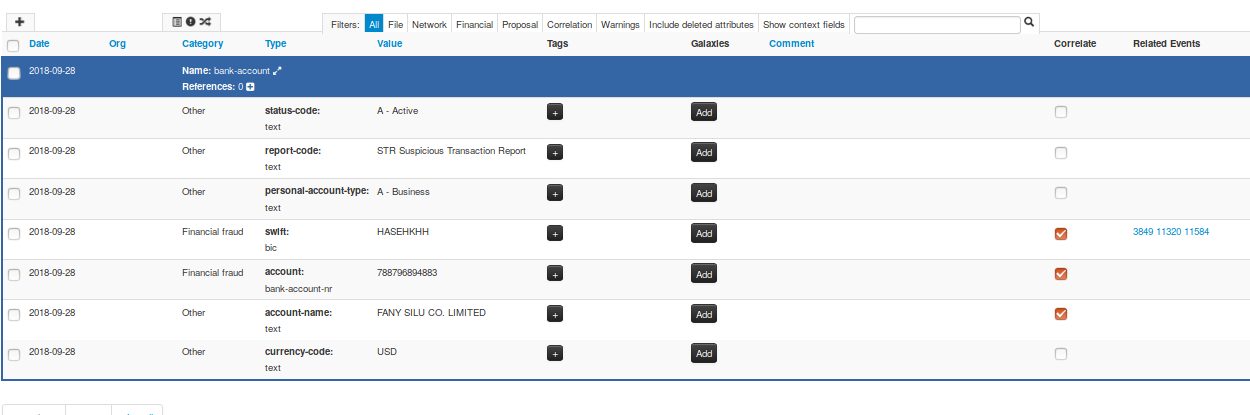
\includegraphics[scale=0.24]{screenshots/bankaccount.png}
        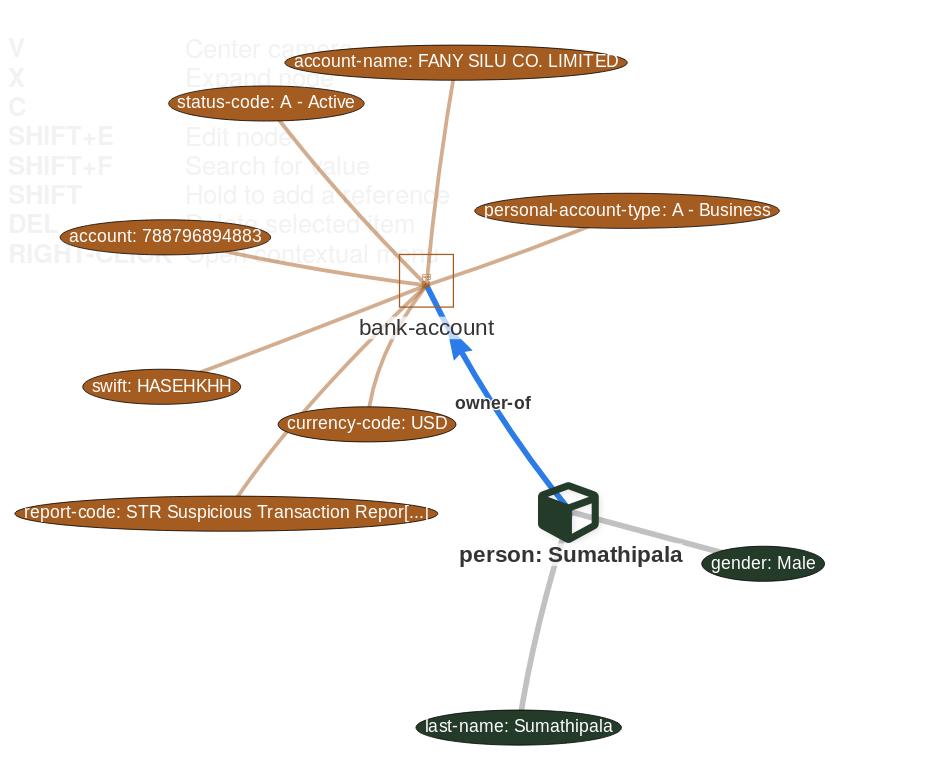
\includegraphics[scale=0.18]{screenshots/bankview.png}
\end{frame}


\begin{frame}
\frametitle{MISP core distributed sharing functionality}
\begin{itemize}
\item MISP is a {\bf peer to peer} sharing software
\item As such, everyone can be a {\bf consumer} and/or a {\bf producer} of information.
\item Immediate benefit without the obligation to contribute.
\item Low barrier of entry to get acquainted with the system.
\end{itemize}
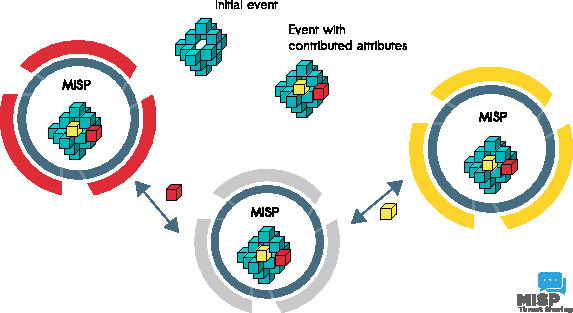
\includegraphics[scale=0.9]{misp-distributed.pdf}
\end{frame}

\begin{frame}
\frametitle{Information quality management}
    \begin{itemize}
        \item Correlating data
        \item Feedback loop from detections via {\bf Sightings}
        \item {\bf False positive management} via the warninglist system
        \item {\bf Enrichment system} via MISP-modules
        \item {\bf Integrations} with a plethora of tools and formats
        \item Flexible {\bf API} and support {\bf libraries} such as PyMISP to ease integration
        \item {\bf Timelines} and giving information a temporal context
        \item Full chain for {\bf indicator life-cycle management}
    \end{itemize}
\end{frame}

\begin{frame}
    \frametitle{Modelling new data structures for COVID-19}
    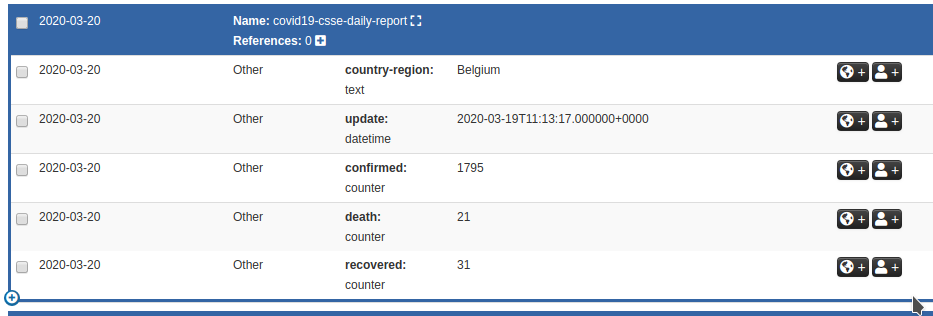
\includegraphics[width=1.00\linewidth]{covidobject.png}
    We are rapidly building new models for the different COVID-19 related information sources
\end{frame}

\begin{frame}
    \frametitle{Demo time}
    \begin{itemize}
        \item View data
        \item Dashboards
        \item Create medical data
        \item Create cyber security data
    \end{itemize}
\end{frame}

\begin{frame}
\frametitle{How can you get involved?}
    \begin{itemize}
        \item Join the COVID-19 community
        \item Either just use the data, or contribute data back, examples:
        \begin{itemize}
            \item Ongoing Covid-19 phishing campaigns
            \item Sharing warninglists of known valid covid-19 related websites
            \item Local articles about the situation in your area
            \item Best practice recommendations
            \item Informations on travel restrictions
        \end{itemize}
        \item Create {\bf pull requests}
        \item Share your ideas
    \end{itemize}
\end{frame}

\begin{frame}
  \frametitle{Contact us}
  \begin{itemize}
    \item \url{https://www.misp-project.org/}
    \item \url{https://www.misp-standard.org/}
    \item \url{https://github.com/MISP}
    \item \url{info@misp-project.org}
    \item \url{https://twitter.com/MISPProject}
  \end{itemize}
\end{frame}


